\chapter{Agglomerative clustering algorithms}

\todo{uplne nejdriv je potreba ukazat priklady k cemu je vlastne clusterovani, minimalne urcite predtim nez se vrhnes na dissovani clusterovych vedcu za to ze nemaji striktni definici klastru :D intro idealne ukaze priklady k cemu je clusterovani (je to redukce datasetu na nekolik vyrazne jednodussich disjunktnich casti, ktery maj vetsinou nejakou vhodnou vlastnost, napr. jsou kompaktni nebo vzajemne dost podobny)}
In the field of clustering analysis, there is no strict definition for a cluster itself. That may be one reason why there is such a vast amount of clustering algorithms; many authors such as \citet{estivill2002so} discuss this topic.  \xxx{However}\todo{however znamena `jenze bohuzel'}, the~one \xxx{think} in common that we can find among all the algorithms \xxx{is a work} with a~group of data objects.

\xxx{According to a field of use,} the data objects are represented variously (graphs, text sequences, etc.). The current thesis will focus on a clustering of objects represented by a vector of real numbers.

Suppose a dataset $\mathcal{D}$ given as a $n$ $d$-dimensional vectors $(x_1,\dots,x_d) \subset \R^d$  --- objects; each element of a vector describes a specific object property. Two objects are similar if values of their respective properties are alike. Then, a clustering analysis can be defined as a form of an object grouping into subsets of $\mathcal{D}$ that maximizes the inter-set object similarity and minimizes the intra-set object similarity.

\section{Clustering models}

\todo{tech modelu je 9000+, udelat tady seznam kterej vypada jako kompletni je trochu nebezpecny. Proste napis ze tech modelu je vic, a ukazes jeden centroidni, a pak se budes venovat hierarchickejm.}
Specific variations of clustering analysis are defined by a clustering model. For the~purpose of the following chapters, we will describe these two clustering models:
\begin{itemize}
	\item Centroid-based model
	\item Hierarchical model
\end{itemize}


\subsection{Centroid-based model}

\emph{The centroid-based clustering model} represents clusters only by a central vector --- \clen\emph{centroid} --- which is not necessarily a member of a dataset.

\todo{zadefinuje ty veci co pouzivas dal (konkretne na zacatku tvrdis ze nikdo vlastne nezna presnou definici clusteru (pritom zna) a pak to pouzivas v definici jako neco uplne v pohode definovanyho}
\begin{defn}[Centroid]
	Given a cluster $\mathcal{C} \subset \R^d$, we define the \emph{centroid} $c \in \R^d$ of the cluster $\mathcal{C}$ such that its $i$-th element is equal to the arithmetic mean of the $i$-th elements of all points $o \in \mathcal{C}$. \todo{semantickej rejp: neni to v $k$-means nahodou obracene, ze drzis centroidu a k ni prilepis vsechny body ktery ji maj nejbliz?}
	\label{def01:centr}
\end{defn}

Many~implementations of this model need the number of required centroids in advance (denoted by $k$). We define the following optimization problem for~this kinds of~algorithms: \todo{jen hint: v anglictine neplati pravidlo ze `predlozka na konci radku nesmi bejt sama'.}

\begin{problem}[Centroid-based clustering]
	Having a distance function $d$, find $k$ centroids $C_1,\dots,C_k$ from the domain of the dataset $\mathcal{D}$ such that the sum \ref{eq01:sum}
	is minimized.
\end{problem}

\begin{equation}\label{eq01:sum}
	\sum_o^{\mathcal{D}} \min_{i=1\dots k}d(o,C_i)
\end{equation}

This problem is \xxx{uneasy} to solve due to its exponential complexity\todo{ref? btw ma to presnej nazev}. Hence, many approximation algorithms emerged. 

\subsubsection{k-means}

\todo{obecna rada: jakmile mas nekde subsubsection, potrebujes ty kapitoly preusporadat :D}
The most common implementation of a centroid-based clustering is \emph{k-means}. Its algorithm can be expressed in a few simple steps (see alg.~\ref{alg01:kmeans}).
\todo{v tom algoritmu rozhodne neni `few simple steps', zkus to vyjadrit mnozinove misto explicitnima cyklama. $k$-means by mel zabrat tak 6 radku.}

\begin{algorithm}[t]
	\caption{$k$-means clustering \xxx{Sazet algoritmy do textu je pekne hnusny (konkretne tady to ten text na strance rozseklo na 1 radek nahore a 1 radek dole, cist neco takovyho boli), vzdycky k nim dej aspon [t] at se vysazej nahoru na stranku.}}
	\label{alg01:kmeans}
	\begin{algorithmic}[1]
		\Procedure{$k$-means}{$k\in\R$, $\mathcal{D} \subset \R^d$, $d \in \R^d \times \R^d \to \R$}
		\State $\mathcal{C} \gets$ first $k$ objects from  $\mathcal{D}$ \Comment{select initial centroids}
		\Repeat
			\For{$i \in \{1\dots k\}$}
				\State $K_i \gets \{\}$\Comment{create empty clusters}
			\EndFor
			\ForAll{$o \in \mathcal{D}$}
				\State $j \gets$ index of the closest centroid $c_j \in \mathcal{C}$ to $o$; $d(o,c_j)$ is minimal
				\State $K_{j} \gets K_{j} \cup o$ \Comment{assign objects to clusters}
			\EndFor
			\For{$i \in \{1\dots k\}$}
				\State $c'_i \gets$ centroid of $K_i$ \Comment{compute new centroids}
			\EndFor
			\State $\mathcal{C}' \gets \{c'_1,\dots,c'_k\}$
			\State swap $\mathcal{C}$ and $\mathcal{C}'$
		\Until{$\mathcal{C} = \mathcal{C}^\prime$}
		\State \textbf{return} $\mathcal{C}$
		\EndProcedure
	\end{algorithmic}
\end{algorithm}


The algorithm divides data into $k$ clusters (hence, \emph{k}\todo{tady to k chces psat jako $k$, emph je emphasis}-means\todo{a proc v tom nazvu jsou means?}) in an iterative manner. Before the first iteration, initial $k$ central vectors are selected from the~dataset (we chose the first $k$ objects; however, the way of selecting $k$ initial vectors varies between 
implementations). In the iteration loop, dataset objects are grouped into clusters according to the closest centroid. After that, new centroids are computed from new clusters. Next iteration follows until centroids does not change or a predefined number of iterations is reached. 

The $k$-means algorithm is easily comprehensible\todo{to whom?}; hence, it can be employed in a large variety of datasets\todo{to ze je algoritmus jednoduse pochopitelnej moc neimplikuje ze by sel pouzivat na hodne datasetu}. Moreover, the algorithm simplicity favors in its great performance\todo{hodne nepresny}. However, \xxx{the disadvantages are inability} to deal with the noise in~a~dataset and clusters of a non-convex shape~\cite{uppada2014centroid}.\todo{tohle `zhodnoceni' je mozny vyrazne zlepsit tim ze rovnou rejpnes PROC jsou ty implementace jednoduchy a rychly, a ukazes priklad proc prirazeni clusteru podle centroid tem nekonvexnim tvarum moc nefandi. (hint: voronoidy jsou konvexni ve vsech dimenzionalitach)}
  

\subsection{Hierarchical model}

In the \emph{hierarchical clustering model}\todo{neprehanej ten emph}, objects are \emph{connected} together forming a tree-like structure. In contrast with the aim of a centroid-based model that returns only $k$ centroids, hierarchical clustering algorithms capture the whole connecting process. These algorithms start with all objects from a dataset as initial clusters. Each iteration, two clusters are connected creating a new one, finishing with one all-inclusive cluster. Commonly, the algorithms represent the connecting process as an ordered list of pairs --- a list of connected clusters~\cite{karypis1999chameleon}.

\todo{Tohle chces uvyst ze `rozlisujeme 2 zakladni metody jak vyrobit dendrogram'}The above described approach of a hierarchical algorithm is called \emph{agglomerative} approach. An agglomerative algorithm begins with each object representing a cluster on its own. Then, in a bottom-up fashion, clusters are successively connected into the only cluster. The other option is \emph{divisive approach}. Beginning with a single all-inclusive cluster it is divided into sub-clusters until single objects remain~\cite{rokach2005clustering}. 

The result of a hierarchical clustering can be viewed \xxx{in} a \emph{dendrogram} (see fig.~\ref{fig01:dendro}). The x-axis states the \xxx{distance}\todo{neni to obecna metrika? nebo podobnost? vklidu si zadefinuj `similarity metric'.}\ between connected clusters. The y-axix shows labels of the objects from a dataset\todo{fakt Y?}. Hence, the clusters that are connected in the higher part of the dendrogram \xxx{were}\todo{`muzou byt povazovany za mene podobne'}\ further apart from each other, and the~clusters connected at its bottom \xxx{were close} to each other. \todo{jakej to je dataset? co do toho slo za data? Proc tam je Wyoming ale neni tam Frydek-Mistek?}

\begin{figure}\centering
	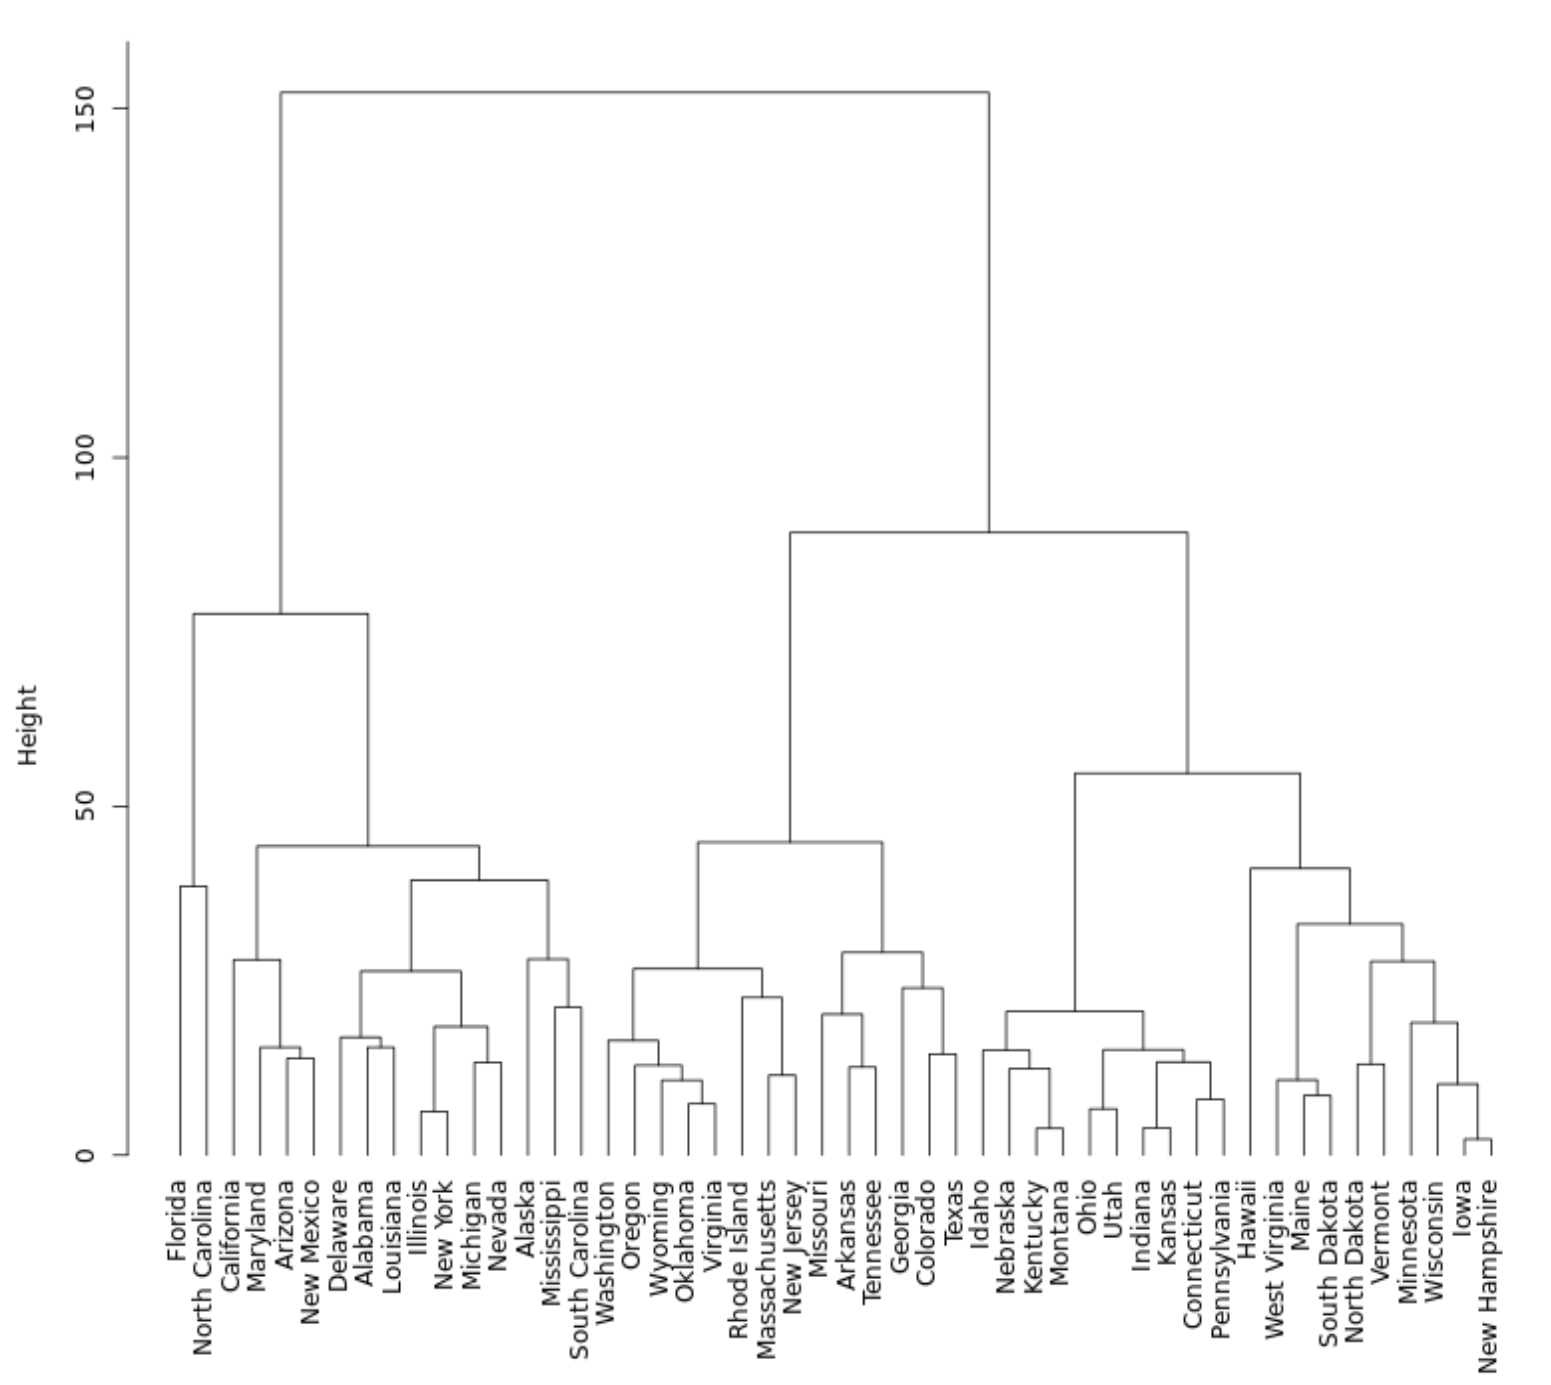
\includegraphics[width=10.5cm]{img/dendro}
	\caption{An example of a dendrogram. \xxx{Odkud je ten obrazek, pripadne jak jsi ho vyrobil? Jak jednoduse interpretovat ty data co v nem jsou videt?}}
	\label{fig01:dendro}
\end{figure}

To know which two clusters are connected (or respectively, how a cluster is~divided into two), algorithms use a \emph{measure of a dissimilarity} between clusters.  
A~hierarchical clustering model distinguishes various kinds of algorithms based on~the~choice of this measure. Commonly, the computation of the measure is~dependent on the two factors: a \emph{distance function} and a \emph{linkage criterion}. 

\subsubsection{Distance functions}

A \emph{distance function} is used on objects of a dataset to \xxx{express}\todo{measure? Mozna fakt zacni vejs tim ze si vyrobis dissimilarity measure a vzdalenost pak prohlasis za jednu moznou metriku ktera na to jde pouzit}\ how far they are~from each other in the observed domain. \xxx{Supposing objects are represented}\todo{Pokud jsme dataset schopny popsat jako mnozinu ...}\ as vectors $v \in \R^d$, variations of \emph{Minkowski distance formula} (see eq.~\ref{eq01:mink}) are the most commonly used.\todo{ref? konkretne nechces tvrdit ze jsou nejvic pouzivany (protoze nejsou), ale muzes tvrdit ze z minkowskeho vzdalenosti jde ten dissimilarity vyrobit velice jednoduse a rychle. Pridej si tam kosinovku.}
They are \emph{Manhattan distance} ($p=1$), \emph{Euclidean distance} ($p=2$) and \emph{Chebyshev distance} ($p \to \infty$) (see tab.~\ref{tab01:mink}).

It is obvious that the choice of a distance function can influence the result of~a~clustering\todo{not at all, ref?}. \xxx{Hence,} it\xxx{what exactly?}\ should be chosen with respect to the properties of~a~provided dataset. \citet{aggarwal2001surprising} show the qualitative behavior of different distance functions in the $k$-means algorithm.\todo{tohle chces rewordovat aby bylo jasny ze to vysvetluje predchozi vetu}

\begin{equation}\label{eq01:mink}
||a-b||_p = (\sum_{i=1...d}|a_i-b_i|^p)^{\frac{1}{p}}
\end{equation}

\begin{table}[t]
	\centering
	\renewcommand{\arraystretch}{1.3} %XXX: tohle se dost hodi
	\begin{tabular}{ll}
		\toprule
		Distance measure & Formula \\
		\midrule
		Manhattan & $\|a-b\|_1 = \sum_{i}|a_i-b_i|$          \\
		Euclidean & $\|a-b\|_2 = \sqrt{\sum_{i}(a_i-b_i)^2}$ \\
		Chebyshev & $\|a-b\|_\infty = \max_{i}|a_i-b_i|$  \\
		\bottomrule
	\end{tabular}
	\caption{Variations of the Minkowski distance formula.}
	\label{tab01:mink}
\end{table}

\subsubsection{Linkage criteria}

\xxx{As the reader may have already discovered, one particular problem arises.} A~hierarchical algorithm can not compute \xxx{a} proximity of two clusters only by a distance function as it is the function of~\emph{dataset objects}. Hence, we define a~function of~\emph{object clusters} to \xxx{complete} the process of measuring dissimilarity\todo{ale nikde neni oznaceno ze nejakej proces zacal?}; a~\emph{linkage criterion}\todo{Mozna chces jasne rict ze tohle popisuje hromady moznosti jak zmerit vzdalenost dvou SKUPIN bodu, coz je problem kterej pomerne prirozene vznika kdyz ty body lepis}. Given clusters $A$ and $B$ as sets of dataset objects and a distance function~$d$, we define the following \emph{linkage criteria}\todo{moc emph, navic nikde nedefinujes proc se mereni vzdalenosti 2 skupin bodu vlastne rika linkage criterion}~\cite{yim2015hierarchical} (see fig.~\ref{fig01:link}):

\begin{description}
	\item[Single linkage] -- \xxx{Also referred to as the minimum method}, the \emph{single linkage criterion}\todo{moc emph}\ computes the distance between $A$ and $B$ as the minimum distance between all pairs $(a,b) \in A\times B$ (see eq.~\ref{eq01:single_link}).
	\begin{equation}\label{eq01:single_link}
	\min\{d(a,b) : a \in A, b \in B\}
	\end{equation}
	
	The major drawback this criterion suffers is the \emph{cluster chaining}. \xxx{Such two}\todo{which two?}\ clusters can be connected that they do not share any other pair of close proximity objects than the one that determined the connection. This produces long thin clusters with \xxx{a great}\todo{great znamena `skvely'. Tady ta vzdalenost neni moc skvela.} distance between some objects.
	
	\item[Complete linkage] -- Also referred to as the maximum method, the \emph{complete linkage criterion} is similar to the single linkage criterion. But as opposed to~finding the minimum, this criterion uses the maximum of object pairs for the~computation of a cluster dissimilarity (see eq.~\ref{eq01:complete_link}). 
	\begin{equation}\label{eq01:complete_link}
	\max\{d(a,b) : a \in A, b \in B\}
	\end{equation}
	
	The criterion suffers from its simplicity as well as the single linkage. But~instead of naively connecting dissimilar clusters, here similar clusters are~not connected in some cases. Having all object pairs in a close proximity to each other but one object being rather far from the others, the~criterion will not link the clusters as the maximum distance deteriorates the rest.
	
	\item[Centroid linkage] -- The \emph{centroid linkage criterion} tries to solve the problems of~the~aforementioned criteria by measuring the distance between the centroids of clusters. It~introduces a form of an average into the computation; the think that the criteria above lack.
\end{description}

The choice of a linkage criterion in hierarchical clustering algorithm is vital. As~stated above, it can change the course of clustering in a great manner. Chosen improperly, it can have a disastrous effect on the final result.

\begin{figure}\centering
	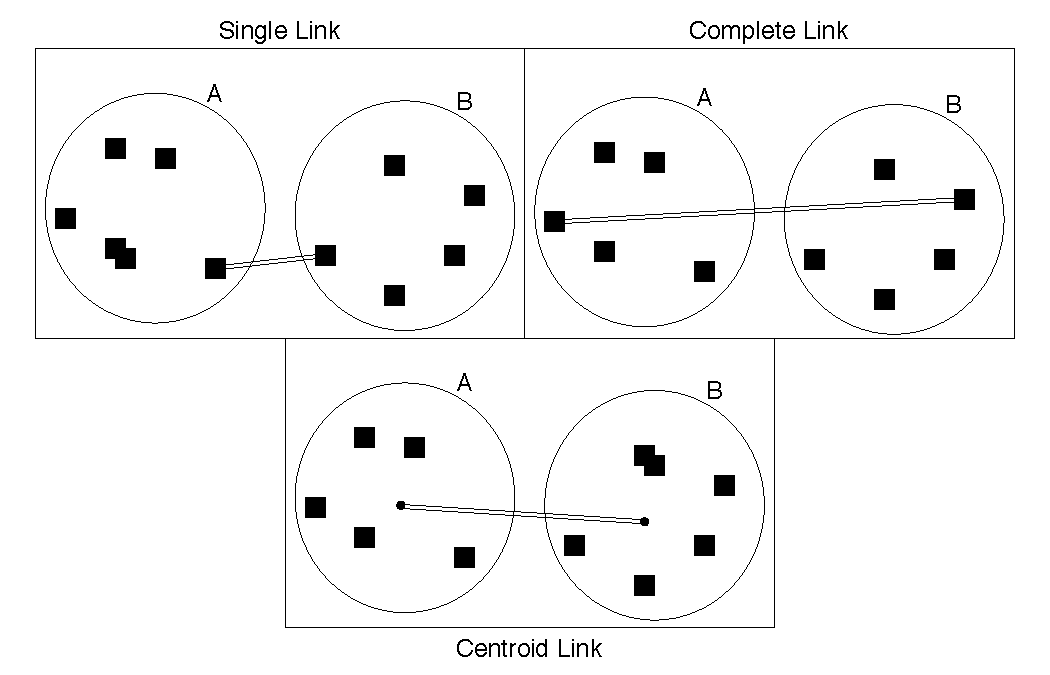
\includegraphics[width=10cm]{img/linkage_criteria}
	\caption{An example of three linkage criteria. The double line represents the~distance between clusters A and B according to the respective criterion. \xxx{tohle by si zaslouzilo presazet v tikzu, idealne tak aby ty pismena mely jeste citelnou velikost. V tom better-mff-thesis mam example kterej by moh pomoct.}}
	\label{fig01:link}
\end{figure}

\section{Mahalanobis-based hierarchical clustering}

\todo{nadpis upravit na `Mahalanobisovsky lepeni clusteru v hierarchickym clusterovani'. Bacha na spravnej nazev ty metody, Mahalanobis-based znamena zes do toho umlel kus nejakyho inda. Spravne to je `Mahalanobis‐average linkage h. cl.'}
To produce more meaningful results\todo{neukazals problem a rejpes do toho ze vysledky nejsou meaningful, chce to priklad. Muzes si vzit obrazky od Siegera z paperu nebo z githubu (a spravne je ocitovat)}, hierarchical clustering algorithms have branched into many variations; each focusing on a specific dataset type. The~\emph{Ma\-ha\-la\-no\-bis-based hierarchical clustering analysis} (MHCA) focuses on the datasets that create clusters of ellipsoid shapes. Such datasets are common products of~the~measurements of cell cytometry data in bio\xxx{-}informatics.\todo{mozna `which was the original purpose for the design}. \xxx{tady fakt hodne chybi reference!}

\subsection{Mahalanobis distance}

\xxx{The} significant part\todo{statistically?}\ of \xxx{this} clustering \xxx{variation} is \xxx{the measure} of the cluster dissimilarity. It is based on the \emph{Mahalanobis distance}~\cite{mahalanobis1936generalized}, a~distance between a~point and a set of points (in our case a cluster). If points in the set are strongly correlated in some axis, then points laying on this axis are closer to the set than points that are not; even if their euclidean distance to the center of the set is closer.

For \xxx{its computation, the Mahalanobis distance uses}\todo{timhle rikas ze ta vzdalenost je akter kterej se pocita sam, ve skutecnosti moc ziva neni}\ the covariance matrix of~a~participating cluster. \xxx{To know how the matrix is created, we need to~define the \emph{random vector of a cluster} first.}\todo{tohle nedava moc smysl}

\begin{defn}[Random vector]\todo{tahle definice nevypada ze by se nekde vubec pouzivala?}
	Given a cluster of $d$-dimensional points $\mathcal{C} \subset \R^d$, we define the \emph{random vector} $v$ of the cluster $\mathcal{C}$ as a vector of $d$ discrete random variables; a random variable $v_i$ has equal probability values $\{o_i:o\in \mathcal{C}\}$
\end{defn}

Using the random vector of a cluster we can easily create the covariance matrix of a cluster and properly define the Mahalanobis distance:\todo{kde je definice nebo ref kovariancni matice?}

\begin{defn}[Mahalanobis distance]\todo{vkladat equationy s vlastni referenci do definic s vlastni referenci je uplne zbytecny, opravil sem to. Btw trochu jsem poopravil ty vzorecky, prolez si to s \texttt{git diff --word-diff}} 
	\label{eq01:maha}
	Having a cluster of $d$-dimensional points $\mathcal{C} \subset \R^d$, its centroid $c$ and the covariance matrix $\mathcal{S}$, we define the \emph{Mahalanobis distance} between $u \in \R^d$ and $\mathcal{C}$ as
	\[d_\text{Maha}(u,\mathcal{C}) = \sqrt{(u-c)^TS^{-1}(u-c)}.\]\todo{kovariancni matice se bezne znacej jako $\cov(\mathcal{C})$, kdyz uz to chces takhle jako funkci.}
\end{defn}


However, using the equation \ref{eq01:maha}, we are only able to compute a \emph{point-cluster}\todo{emphhhhh, jinak jde to napsat i bez pomlcky pekne po slovech a bude to pochopitelnejsi. Nepouzivej proximity ale distance.} proximity. To fully incorporate the distance in a hierarchical algorithm, we need to find a method how to measure \emph{cluster-cluster} proximity. There are two options how to achieve this:

\todo{ten itemize tady nedava vubec smysl, optiony vyjmenuj na zacatku (i s vysvetlenim) at to je jasny hned,}
\begin{itemize}

\item
First, we can choose a path of the single and complete linkage criterion; hence, all points in cluster contribute to the measure. We achieve this with~the~\emph{Full Mahalanobis distance} (FMD):

\begin{defn}[Full Mahalanobis distance]
	Having clusters $\mathcal{C}$ and $\mathcal{C}'$, we define the \emph{Full Mahalanobis distance} between clusters $\mathcal{C}$ and $\mathcal{C}'$ as the arithmetic mean of the Mahalanobis distances between each object $o \in \mathcal{C}$ and the~cluster $\mathcal{C}'$ \xxx{(see eq.~\ref{eq01:fmd})}.
	\begin{equation}\label{eq01:fmd}
	d_\text{MahaFull}(\mathcal{C},\mathcal{C}') =\frac{1}{|\mathcal{C}|}\sum_{o\in\mathcal{C}}{d_M(o,\mathcal{C}')}
	\end{equation}
	\label{def01:fmd}
\end{defn}

\item
The \xxx{second option}\todo{fakt je druhy? (ma to poradi smysl?)}\ is similar to the centroid linkage as only the centroid of a cluster takes part in the computation. We define \xxx{this} as the \emph{Centroid Mahalanobis distance} (CMD):

\begin{defn}[Centroid Mahalanobis distance]
	Having a cluster $\mathcal{C}$ with its centroid $c$ and a cluster $\mathcal{C}'$, we define the \emph{Centroid Mahalanobis distance} between clusters $\mathcal{C}$ and $\mathcal{C}'$ as the Mahalanobis distance between $c$ and $\mathcal{C}'$ \xxx{(see eq.~\ref{eq01:cmd})}.
	\begin{equation}\label{eq01:cmd}
	d_\text{MahaCentroid}(\mathcal{C},\mathcal{C}')=d_\text{Maha}(c,\mathcal{C}')
	\end{equation}
	\label{def01:cmd}
\end{defn}

\end{itemize}

To illustrate the measure of the Mahalanobis distance, let us suppose we have two elliptic clusters. In the means of the proximity, the measure favors such clusters that their ellipsis are alongside rather than in a prolongation of one another~\cite{dagnelie1991using} (see fig.~\ref{fig01:ellipses}). Only when the objects of a cluster form a spherical shape, this measure of dissimilarity is proportional to the euclidean distance with a corresponding linkage.

\begin{figure}\centering
	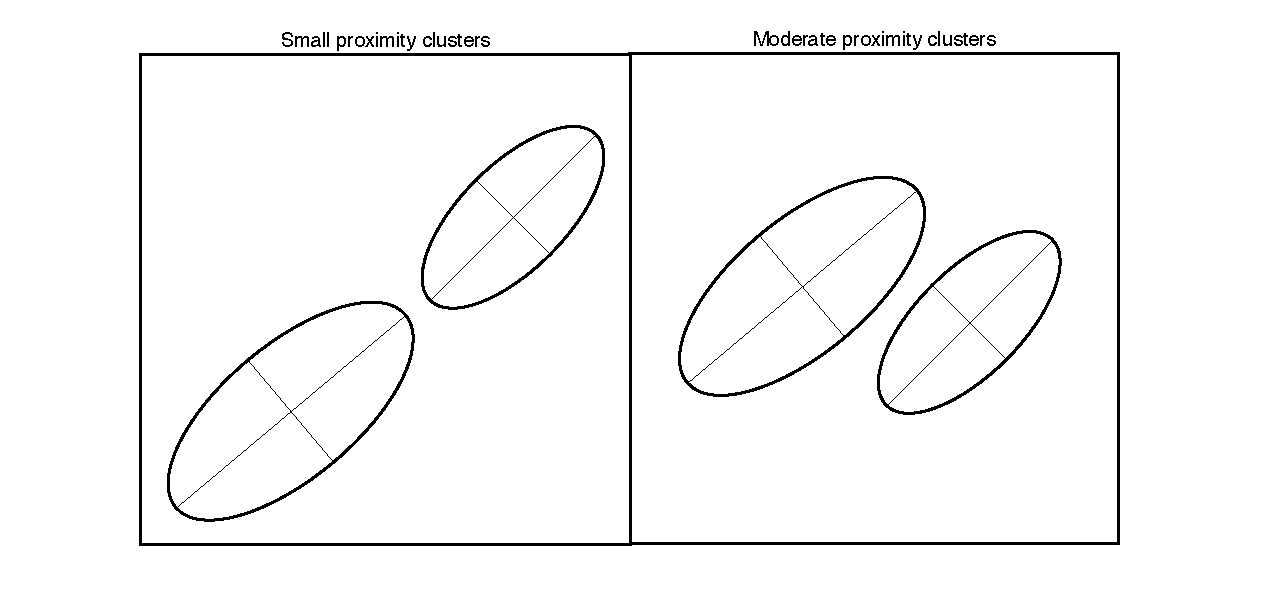
\includegraphics[width=10cm]{img/ellipses}
	\caption{An example of the cluster dissimilarity in the Mahalanobis-based hierarchical clustering.}
	\label{fig01:ellipses}
\end{figure}



The pros and cons between FMD and CMD are trivial. Due to the full point contribution, FMC can produce more precise measure than its simpler counterpart. On the~other hand, CMD compensates this with much lower time complexity.

\vspace{0.5cm}

To make use of these Mahalanobis distance variants in MHCA implementations, we need the distance function to be \emph{symmetric}\todo{eeeeeeeeeeemph}. Originally, the Mahalanobis distance is not a symmetric function. \xxx{However}\todo{Co radsi `fortunately'?}, we easily \xxx{achieve this attribute}\todo{Achievement unlocked! neni to attribute ale property, a chces vklidu rict ze ji mirne upravis nebo pofixujes, ne ze achievujes :D}\ with the \emph{Generalized distance}.

\begin{defn}[Generalized distance]
	Given clusters $\mathcal{C}$, $\mathcal{C}'$ and a variant of~the~Mahalanobis distance~$d$ (either FMD or CMD), we define the \emph{Generalized distance} between clusters $\mathcal{C}$ and $\mathcal{C}'$ as the arithmetic mean of distances between $\mathcal{C}$, $\mathcal{C}'$ and $\mathcal{C}'$, $\mathcal{C}$ \xxx{(see eq.~\ref{eq01:gene})}.
	\begin{equation}\label{eq01:gene}
	d_\text{Variant}(\mathcal{C},\mathcal{C}') = \frac{d_\text{Variant}(\mathcal{C},\mathcal{C}')+d_\text{Variant}(\mathcal{C}',\mathcal{C})}{2}
	\end{equation}
	\label{def01:gene}
\end{defn}  


\subsection{Algorithm behavior improvements}

If the distance function of a MHCA implementation was let to be the pure Mahalanobis distance, it would eventually halt due to the following problem --- the~covariance matrix computation.

In early stages of MHCA --- when clusters consist of fewer points --- the covariance matrix of a cluster is often singular. Hence, we can not compute its inverse and perform the distance measure. Furthermore, the matrix can happen to be close to singular and --- when inverted --- can produce distorted results.

To solve this problem, we used the~euclidean distance with the~centroid linkage on clusters whose sizes are under a~specified threshold --- the~\emph{Mahalanobis threshold}. The value of the threshold is proportional to the size of a dataset~\cite{fivser2012detection}. Hence, to implement this optimization we defined the \emph{Altered general distance}.

\begin{defn}[Altered general distance]
	Given a threshold $T_M$, a cluster $\mathcal{C}$ with~its centroid $c$, a cluster $\mathcal{C}'$ with~its centroid $c'$ and a variant of the Mahalanobis distance~$d$ (either FMD or CMD), we define the \emph{Altered general distance} by the equation \ref{eq01:alt}.
	\begin{equation}
	d_A(\mathcal{C},\mathcal{C}')=
	\begin{cases}
	d_G(\mathcal{C}, \mathcal{C}'), & \text{if $|\mathcal{C}|\ge T_M$ and $|\mathcal{C}'|\ge T_M$},\\
	\dfrac{d(\mathcal{C}, \mathcal{C}')+||c-c'||_2}{2}, & \text{if $|\mathcal{C}| < T_M$ and $|\mathcal{C}'|\ge T_M$},\\
	\dfrac{||c-c'||_2+d(\mathcal{C}', \mathcal{C})}{2}, & \text{if $|\mathcal{C}|\ge T_M$ and $|\mathcal{C}'|< T_M$},\\
	||c-c'||_2, & \text{if $|\mathcal{C}|< T_M$ and $|\mathcal{C}'|< T_M$}.\\
	\end{cases}
	\label{eq01:alt}
	\end{equation}
	\label{def01:alt}
\end{defn}



\section{Complexity comparison of hierarchical clustering algorithms }

\todo{nadpis: chces Computational complexity of ...}
The common problem in clustering algorithms is their time complexity. In hierarchical clustering algorithms, we can \xxx{achieve} time complexity of $O(n^3)$ using $O(n^2)$ space\todo{unsupported claim}. \xxx{However,} this restricts the use of the algorithms; datasets must consist of $10^3$ to $10^5$ points \xxx{when} using \xxx{a} contemporary hardware. Note that this restriction is present not only due to the time complexity; for the current computers, it would be a difficult task to store $10^6$ data points into a structure with quadratic space requirements (i.e. a matrix).\todo{tohle ve skutecnosti neni uplne pravda, 4TB disku/ramky je docela beznej jev}

Due to the consequences of this problem, a MHCA algorithm implementation must be \xxx{created wisely}\todo{tohle muze znamenat cokoliv}. \citet{day1984efficient} help us\todo{fakt pomohli primo nam?! mozna chces rovnou rict ze navrhli vic implementaci}\ with this task by~proposing three different implementations of a hierarchical clustering analysis (HCA). We describe them thoroughly and research potential \xxx{pros and cons they bring}:

\todo{tenhle description je tradicne moc dlouhej, dej na zacatek ze moznosti jsou takovyhle a pak je muzes rozepisovat (asi jako subsectiony)}
\begin{description}
	\item[HCA with the dissmilarity matrix] \xxx{--} The first and the most trivial implementation uses the \emph{dissimilarity matrix} $M$.
	
	\begin{defn}[Dissimilarity matrix]
		Suppose a dataset $\mathcal{D}$ divided into clusters $C_1,\dots,C_m$ and a function $d$ as a measure of dissimilarity. Then, the~\emph{dissimilarity matrix} $M$ is $m\times m$ matrix where $M_{ij} = d(C_i,C_j)$.
		\label{def01:dismat}
	\end{defn}

 Unless there remains only one cluster, the current algorithm searches $M$ for~the~closest pair of clusters, stores the pair and updates $M$ (see alg.~\ref{alg01:dismat}).
	
	\begin{algorithm}[t]
		\caption{HCA with dissimilarity matrix}
		\label{alg01:dismat}
		\begin{algorithmic}[1]
			\Procedure{dismat}{$\mathcal{D} \subset \R^d$}
			\State initialize the dissimilarity matrix $M$
			\For{$k=|\mathcal{D}|$ \textbf{\xxx{downto}} $1$}
			\State search $M$ for the closest pair $(i,j)$ \Comment{time: $O(k^2)$}
			\State store cluster pair $(i,j)$ into the merge list \Comment{time: $O(1)$}
			\State update $M$ \Comment{time: $O(k)$}
			\EndFor
			\State \textbf{return} list of merged clusters
			\EndProcedure
		\end{algorithmic}
	\end{algorithm}

	The main cycle in line $3$ repeats $n = |\mathbb{D}|$ times; each iteration the number of clusters is reduced by 1. The search in line $4$ is bounded by $O(n^2)$ time, having its peak in the first iteration when $k=n$. The update in~line~$6$ reflects the deletion of clusters $i$ and $j$ and the addition of the new one. Hence, it needs to perform $k$ new dissimilarity measures for the new cluster (bounded by $O(n)$ during the first iteration as well). As there are $n$~iterations performed, this results in the overall time complexity of $O(n^3)$. 
	
	The space required to store $M$ is $O(n^2)$. As there is no other non-trivial requirement, the overall space complexity is $O(n^2)$ as well. 
	\begin{rem}
		\xxx{However, there is no need to store the matrix at all.}\todo{tohle jde rict vyrazne presnejc}. We can \xxx{choose} to measure a cluster dissimilarity \emph{in-place}. Line $6$ would become redundant and the time complexity of line $4$ would increase by a constant multiplicative factor; hence, the overall time complexity remains the same while the~space complexity becomes $O(n)$.
	\end{rem}
	

	\item[HCA with the nearest neighbor array] -- This algorithm introduces the array of the nearest neighbors.
	
	\begin{defn}[Nearest neighbor array]
		Suppose a dataset $\mathcal{D}$ divided into clusters $C_1,\dots,C_m$ and a function $d$ as a measure of dissimilarity. Then, the~\emph{nearest neighbor array} $N$ is a $m$-element array of indices $\{1,\dots,m\}$ where each element $N_i$ \xxx{satisfies the equation \ref{eq01:neigh}.}
		\begin{equation}
		d(C_i,C_{N_i}) = \min\{d(C_i,C_j) : j \in \{1,\dots,m\} \setminus \{i\}\}
		\label{eq01:neigh}
		\end{equation}
		
		\label{def01:neigh}
	\end{defn}
	
	 Instead of the dissimilarity matrix, each cluster is assigned the index pointing to~its closest neighboring cluster. 
	 Compared with the previous algorithm, this algorithm trades the expensive \emph{closest pair search} with the expensive \emph{structure update}  (see alg.~\ref{alg01:neigh}).
	
	
	
	\begin{algorithm}[t]
		\caption{HCA with the nearest neighbor array}
		\label{alg01:neigh}
		\begin{algorithmic}[1]
			\Procedure{neighbor}{$\mathcal{D} \subset \R^d$}
			\State initialize $N$
			\For{$k=|\mathcal{D}|$ \textbf{downto} $1$}
			\State search $N$ for the closest pair $(i,j)$ \Comment{time: $O(k)$}
			\State store cluster pair $(i,j)$ into the merge list \Comment{time: $O(1)$}
			\State update $N$ \Comment{time: $O(k^2)$}
			\EndFor
			\State \textbf{return} list of merged clusters
			\EndProcedure
		\end{algorithmic}
	\end{algorithm}
	
	
	 In line $4$, each closest pair search can be performed in $O(n)$ time as the~array length does not exceeds $n$ elements. However in line $6$, the worst case update of $N$ happens when each cluster resides in the closest neighborhood with the clusters that are being merged (clusters $i$  and $j$). In this case, the~whole array has to be recomputed, which corresponds to~the~computation of the whole dissimilarity matrix. Hence, the time complexity for~this step is $O(n^2)$. To sum up, the overall time complexity is $O(n^3)$ and~the~space complexity is $O(n)$ \xxx{as}\todo{hint: `as' se takhle vetsinou pouziva jen hodne zridka a v uplne specifickejch situacich, doporucuju vetsinu predelat na `because' nebo ty vety obratit tak aby to davalo smysl i bez ty spojky.} $N$ does not have more than linear space requirements.
	 
	 \begin{rem}
	 	Despite \clen equal time complexities\todo{mozna to chces rict uplne jinak: naivni implementace ma sice stejnou komplexitu jako predchozi, ale jednoduchym zlepsenim to jde upravit atd. Urcite to nechces jako remark protoze to je celkem centralni zjisteni.}, this algorithm may outperform the previous one as in the majority of situations the update step in line $6$ does not require the whole array to be recomputed. Moreover, if the~number of elements to be updated remains constant each iteration, the overall algorithm time complexity may be $O(n^2)$. 
	 \end{rem}
	 
	 \item[HCA with priority queues] -- This algorithm takes the advantage of the previous one employing the fast search and combines it with the fast update using \emph{priority queues} (see alg.~\ref{alg01:queue}).
	 Each object from a dataset is assigned a~priority queue constructed from the remainder of the dataset. The priority label of a queued element is a dissimilarity measure between the object and the queued element. 
	 
	 \begin{algorithm}[t]
	 	\caption{HCA with priority queues \xxx{misto downto tam dej proste tecky $\dots$. Nema na zvyraznenym miste bejt $k-1$ ?}}
	 	\label{alg01:queue}
	 	\begin{algorithmic}[1]
	 		\Procedure{queues}{$\mathcal{D} \subset \R^d$}
	 		\ForAll{$o \in \mathcal{D}$}
	 		\State initialize a priority queue from $\mathcal{D} \setminus \{o\}$
	 		\EndFor
	 		\For{$k=|\mathcal{D}|$ \textbf{downto} $1$}
	 		\State search $k$ queues for the closest pair $(i,j)$ \Comment{time: $O(k)$}
	 		\State store cluster pair $(i,j)$ into the merge list \Comment{time: $O(1)$}
	 		\State update \xxx{$k$} priority queues \Comment{time: $O(k\log{k})$}
	 		\EndFor
	 		\State \textbf{return} list of merged clusters
	 		\EndProcedure
	 	\end{algorithmic}
	 \end{algorithm}
 
 	
 	As \xxx{an} operation of retrieving a minimum\todo{hint: vzdycky kdyz pises gerundium, zamysli se esi neni potreba. Ceskoslovensky `Ziskani minima' ma anglicky preklad `Retrieval of the minimum'. `Retrieving the minimum' je `Prubeh ziskavani minima'. `Operation of' je s tou prvni moznosti uplne zbytecny, znamena to skoro neco mezi `surgery' a `navy training'.}\ in a priority queue has $O(1)$ time complexity\todo{asi by chtelo rict jak jsou ty PQ implementovany, protoze tohle je jinak dost fishy}, the search step in line $4$ takes $O(k)$ time (bounded by~$O(n)$ during the first iteration). Next in line $6$, we need two delete and one insert operations (corresponding to deleting two merged clusters and inserting one new). As these operations require $O(\log{n})$ time, we can update $n$~queues in $O(n\log{n})$ time.
 	
 	To sum up, the overall time complexity is $O(n^2\log{n})$. The space complexity is \xxx{back to} $O(n^2)$ \xxx{due to}\todo{due to nepouzivej, vetsinou to znamena ze `nekdo muze za neco negativniho', a ve vetsine pripadu to jde rict vic presne nejak jinak.}\ the linear space requirements of a queue.
 	
 	\begin{rem}
 		Note that this is the only algorithm from the three described that unavoidably requires quadratic space. This may lead to the further restrictions of its usability for large datasets.\todo{ted v tom mam teda zmatek, ten prvni nepotreboval kvadratickou pamet? Mozna by to chtelo ty poznamky trochu lip strukturovat (jako dalsi varianty), a idealne sumarizovat do tabulky, at v tom je trochu prehledno.}
 	\end{rem}

\end{description}

To fully show the disadvantages of a hierarchical clustering algorithm complexity\todo{of what exact variant? on what size of data?}, we measured the R language library function \texttt{hclust}; a frequently used implementation of HCA. It computes the centroid linkage with the euclidean distance and uses the dissimilarity matrix. 

Fig. \ref{fig01:hclust} confirms the above stated polynomial time complexity of the implementation. Moreover, it halted at a dataset size of 47K as the testing machine \footnote{Intel Core i9-8950HK, 32GB RAM} ran out of memory.

In conclusion, the space complexity of HCA can be even more restrictive in the means of the overall algorithm usability than its time complexity. \xxx{We solve this}\todo{Spravny pojmenovani situace: vykon tech algoritmu ma vic faktoru a je potreba je balancovat a tradeoffovat. Taky je fajn do toho zapocitat kolik casu vlastne stoji spocitat tu vzdalenostni funkci --- kdyz to bude neco brutalniho (napriklad podobnost DNA sekvenci), tak se vetsinou fakt vyplati vyrobit ty matici, i kdyz bude giganticka. To ze je vzdalenost vyjadritelna jako Minkowski metric je dost specifickej pripad kterej to fakt hodne zjendodusuje. Nastesti v nasem pripade to jde (navic mahalanobis dava smysl jen na euklidovce, coz by tam taky mohlo jit zminit)}\ by removing high space complexity structures (such as the dissimilarity matrix) for the price of a lower speed while retaining the same asymptotic time complexity.

\begin{figure}\centering
	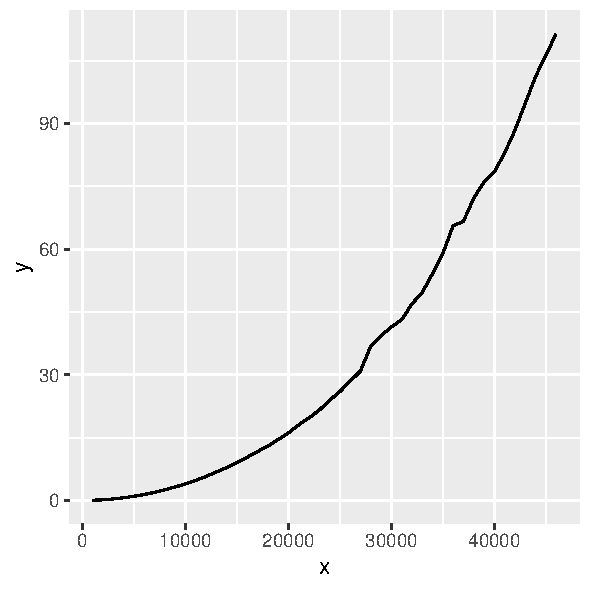
\includegraphics[width=10cm]{img/hclust}
	\caption{Time complexity of \texttt{hclust} with respect to the size of a dataset.}
	\label{fig01:hclust}
\end{figure}
